\documentclass[10pt,a4paper]{article}
\usepackage[latin1]{inputenc}
\usepackage[english]{babel}
\usepackage{amsmath}
\usepackage{amsfonts}
\usepackage{amssymb}
\usepackage{graphicx}
\usepackage{fancyhdr}
\usepackage{lastpage}
\usepackage{multirow}

%Include and define  c code
\usepackage{listings}
\usepackage{color}
\usepackage{textcomp}
\definecolor{listinggray}{gray}{0.9}
\definecolor{lbcolor}{rgb}{0.9,0.9,0.9}
\lstset{
	language=C,
	keywordstyle=\bfseries\ttfamily\color[rgb]{0,0,1},
	identifierstyle=\ttfamily,
	commentstyle=\color[rgb]{0.133,0.545,0.133},
	stringstyle=\ttfamily\color[rgb]{0.627,0.126,0.941},
	showstringspaces=false,
	basicstyle=\small,
	numberstyle=\footnotesize,
	numbers=left,
	stepnumber=1,
	numbersep=10pt,
	tabsize=2,
	breaklines=true,
	prebreak = \raisebox{0ex}[0ex][0ex]{\ensuremath{\hookleftarrow}},
	breakatwhitespace=false,
	aboveskip={1.5\baselineskip},
  columns=fixed,
  upquote=true,
  extendedchars=true,
 frame=single,
 backgroundcolor=\color{lbcolor},
}

\oddsidemargin  -0.5cm
\evensidemargin 0.0cm
\textwidth      17.25cm
\headheight     1.0cm
\headsep		0.7cm
\topmargin      -0.5cm
\textheight		22.0cm

\pagestyle{fancy}
\lhead{Exercise 5}
\chead{EEMB1}
\rhead{\thepage\ of \pageref{LastPage}}
\lfoot{Theis Christensen\\Paulo Fontes\\Dennis Madsen}
\cfoot{Team3}
\rfoot{\today}
\renewcommand{\headrulewidth}{0.4pt}
\renewcommand{\footrulewidth}{0.4pt}
\begin{document}
\part*{EEMB1 - KK - Assignment 5}
Some intro text.
\section{Exercise 1}
A thing to notice here is the use of x++ and ++x. The different between these is that ++x increment x and then returns 
the incremented value, whereas x++ returns x and afterward increments it.\\
In the if statement it first increments the value, which means it checks if 7 is less than 7, this is not true. As the first sentence in the and 
statement is not true, the other is not proceeded. Instead the program proceeds and checks if 8 is below or equal to 9 which is true.\\
Sum up: The if statement is true. The x value has been incremented two times, the output is therefore: \textbf{8}
\section{Exercise 2}
Here a string is putted into the char array dummy. The scanf functions continues reading characters and putting them onto
'dummy' until a 'a' is types. The things putted between the squared brackets contains the characters that the scanf can read, 
and breaks when it reads anything else. The 'in power of sign a' means all characters that is not a can be inputted, and break if a occurs.\\
The output is therefore: \textbf{Life is be}
\section{Exercise 3}
The function could look like this:
\begin{lstlisting}
int IAddOverFlow(int* result, int a, int b)
{			
	if((a+b < INT_MIN) || (a+b >INT_MAX))return 0;		// Overflow
	else
	{
		*result = a+b;
		return 1;					// NO overflow
	}
}
\end{lstlisting}
A simple \textit{if else} is used to check for overflow.\\
Note that INT\_MIN and INT\_MAX should be defined according to the environment where the function is implemented. 
A loop could also be implemented to calculate the values, but would be very time consuming. 
%\begin{figure}[h!]		%Remember to put the h!, to not fuck the sections.
%	\begin{centering}
% 		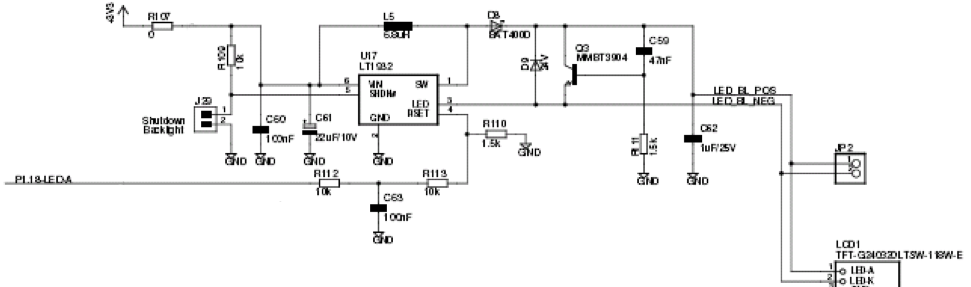
\includegraphics[width=1.0\textwidth]{backlight_circuit}
%		\caption{.}
%	\end{centering}
%\end{figure}

\end{document}
